\section{Module 5: Dynamic Hedging of Impermanent Loss}
\label{sec:module5}

\subsection{LP Payoff, Delta, and Gamma}
\label{sec:module5-theory}

\subsubsection{LP Payoff Shape (Task 5.1.1)}

Let $s(p) = \sqrt{10^{12}/p}$ denote the raw Uniswap sqrt-price for ETH price $p$ (USDC per WETH),
and let $s_a < s_b$ be the position's lower and upper sqrt-price boundaries. For a position with
liquidity $L$, the fee-less LP value is

\[
V_{LP}(p) =
\begin{cases}
  \dfrac{L(s_b - s_a)}{s_a\,s_b\cdot 10^6}, & s(p) \le s_a \quad \text{(above range, all USDC)},\\[8pt]
  \dfrac{L\bigl(s_b - s(p)\bigr)}{s(p)\,s_b\cdot 10^6}
  + p\,\dfrac{L\bigl(s(p) - s_a\bigr)}{10^{18}}, & s_a < s(p) < s_b \quad \text{(in range)},\\[10pt]
  p\,\dfrac{L(s_b - s_a)}{10^{18}}, & s(p) \ge s_b \quad \text{(below range, all WETH)}.
\end{cases}
\]

Figure~\ref{fig:module5-payoff} plots $V_{LP}(p_T)$ for all five positions over
$p_T \in [0.5\,p_0,\;1.5\,p_0]$, alongside the HODL benchmark
$V_{HODL}(p_T) = x_0\,p_T + y_0$.
The vertical gap between the two curves is the impermanent loss.

\begin{figure}[h]
    \centering
    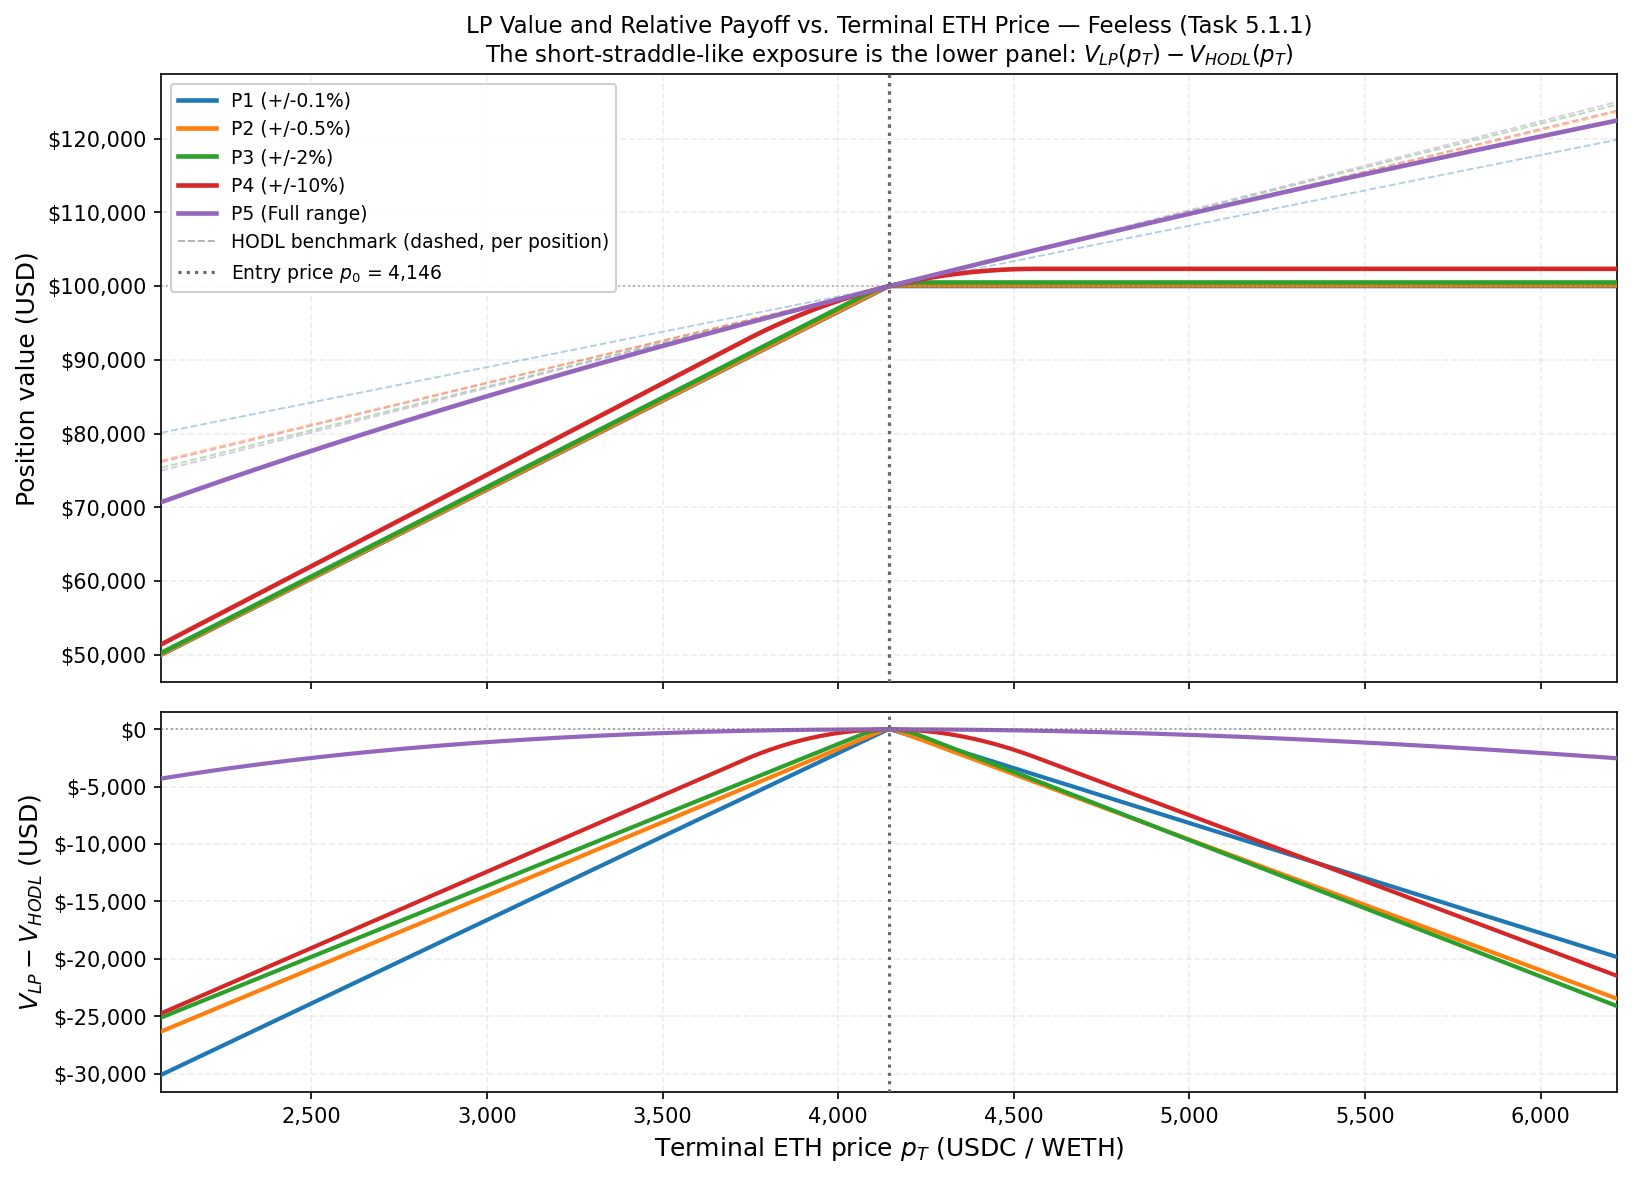
\includegraphics[width=0.9\textwidth]{../data/results/module_5/figures/module5_lp_payoff.png}
    \caption{Fee-less LP payoff (solid) vs.\ HODL benchmark (dashed) for the five representative
             positions over $\pm 50\%$ of the entry price. The gap is the impermanent loss;
             narrower positions suffer larger IL for the same price move.}
    \label{fig:module5-payoff}
\end{figure}

The payoff is concave and resembles a \emph{short straddle}: the LP underperforms the HODL
portfolio for any large move in either direction. The analogy is useful but not exact due to the fact that there is
no upfront premium. Compensation arrives as swap fees only while the price stays within the
active range, and the payoff has finite inventory endpoints rather than the unbounded losses
of a written option.

\subsubsection{Derivation of LP Delta (Task 5.1.2)}

Since $s(p) = (10^{12}/p)^{1/2}$, we have $ds/dp = -s(p)/(2p)$.

\textbf{Above range} ($s(p) \le s_a$): $V_{LP}$ is constant in $p$, so $\Delta_{LP} = 0$.

\textbf{Below range} ($s(p) \ge s_b$): $V_{LP} = p\cdot L(s_b - s_a)/10^{18}$ is linear in $p$,
so $\Delta_{LP} = L(s_b - s_a)/10^{18}$.

\textbf{In range}: Using $p\,s^2 = 10^{12}$ (equivalently, $1/(2p\,s) = s/(2\cdot 10^{12})$),
differentiate each term of $V_{LP}$ with respect to $p$:
\begin{align*}
\frac{d}{dp}\!\left[\frac{L(s_b - s)}{s\,s_b\cdot 10^6}\right]
&= \frac{L}{10^6}\cdot\frac{d}{dp}\!\left(\frac{1}{s}\right)
 = \frac{L}{10^6}\cdot\frac{-1}{s^2}\cdot\frac{ds}{dp}
 = \frac{L}{10^6}\cdot\frac{-1}{s^2}\cdot\!\left(-\frac{s}{2p}\right)
 = \frac{L}{2p\,s\cdot 10^6}
 = \frac{L\,s(p)}{2\cdot 10^{18}},\\[4pt]
\frac{d}{dp}\!\left[\frac{p\,L(s - s_a)}{10^{18}}\right]
&= \frac{L}{10^{18}}\!\left[(s - s_a) + p\,\frac{ds}{dp}\right]
 = \frac{L}{10^{18}}\!\left[(s - s_a) - \frac{s}{2}\right]
 = \frac{L\bigl(s(p)/2 - s_a\bigr)}{10^{18}}.
\end{align*}
Summing: $\Delta_{LP} = L\,s(p)/(2\cdot10^{18}) + L(s(p)/2 - s_a)/10^{18} = L(s(p) - s_a)/10^{18}$.

The complete analytical delta is therefore
\[
\Delta_{LP}(p) =
\begin{cases}
  L\bigl(s_b - s_a\bigr)/10^{18}, & s(p) \ge s_b,\\
  L\bigl(s(p) - s_a\bigr)/10^{18}, & s_a < s(p) < s_b,\\
  0, & s(p) \le s_a.
\end{cases}
\]
In the active range $\Delta_{LP}$ equals the LP's current WETH inventory, which declines
continuously as the price rises (WETH is sold into the pool).

\begin{figure}[h]
    \centering
    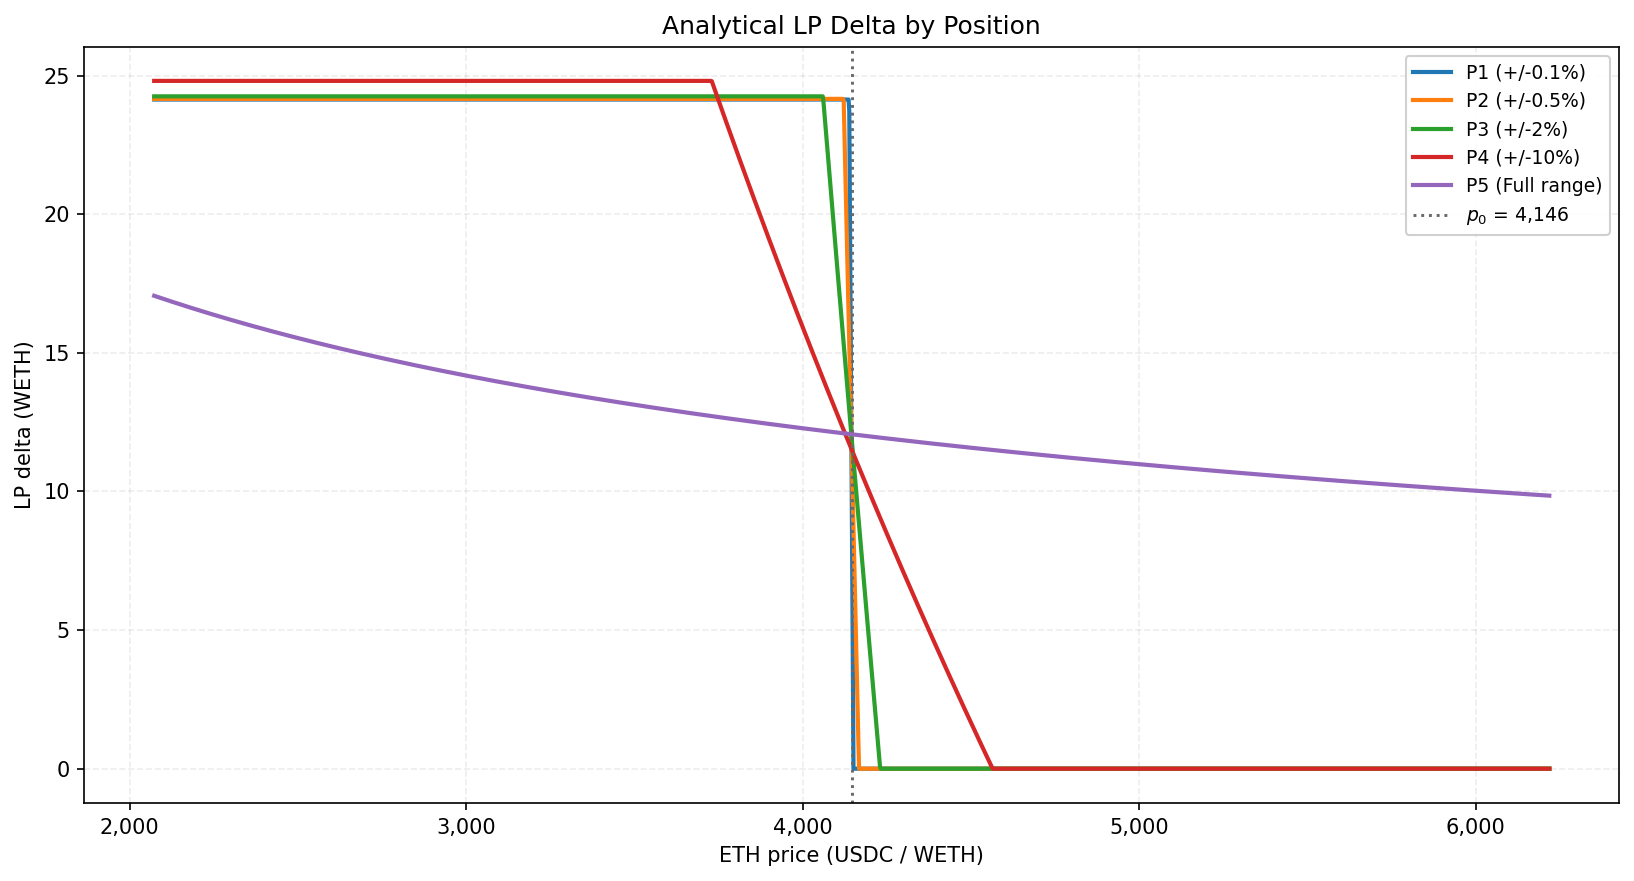
\includegraphics[width=0.9\textwidth]{../data/results/module_5/figures/module5_lp_delta.png}
    \caption{Analytical LP delta by position. Delta is constant below the active range, decreasing
             linearly through it, and zero above.}
    \label{fig:module5-delta}
\end{figure}

\subsubsection{LP Gamma (Task 5.1.3)}

Differentiating $\Delta_{LP}$ once more:
\[
\Gamma_{LP}(p) =
\begin{cases}
  \dfrac{-L\,s(p)}{2p\cdot 10^{18}}, & s_a < s(p) < s_b,\\[6pt]
  0, & \text{otherwise}.
\end{cases}
\]
Gamma is strictly negative inside the active range: the LP is \emph{short gamma}. Its magnitude
$|\Gamma_{LP}| = L\,s(p)/(2p\cdot 10^{18})$ is proportional to $L$. For a fixed notional entry
of \$100\,000, a narrower position requires a larger $L$ to cover a smaller price interval, so
it carries larger $|\Gamma|$ per dollar invested. The wide positions P4 and P5 have the smallest
$|\Gamma|$; P1 (the narrowest, $\pm0.1\%$) has the largest.

\begin{figure}[h]
    \centering
    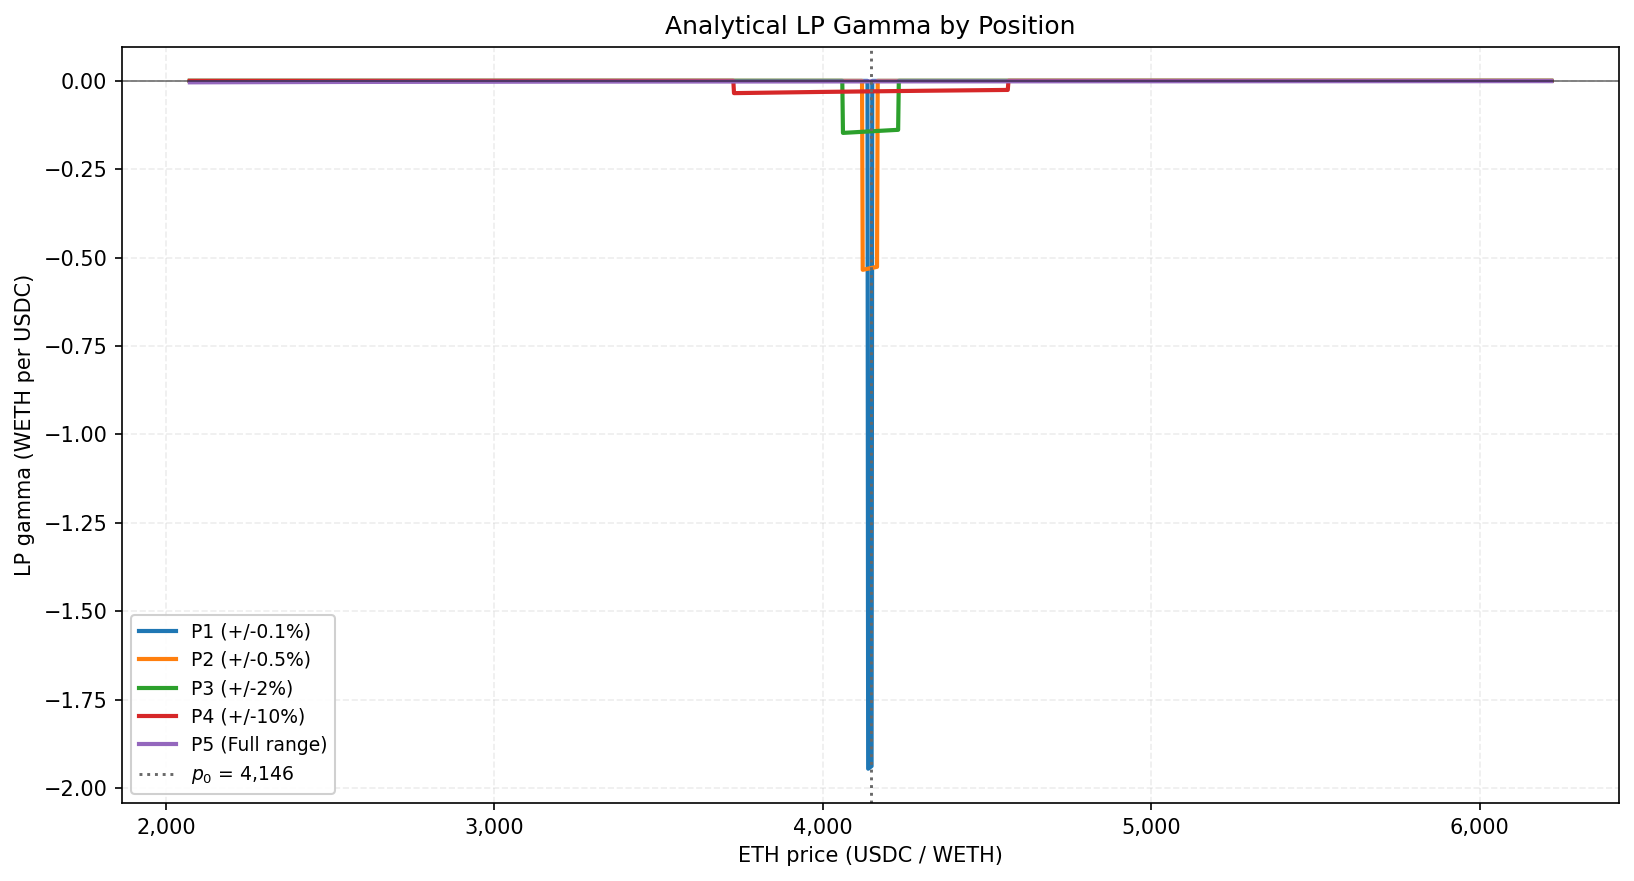
\includegraphics[width=0.9\textwidth]{../data/results/module_5/figures/module5_lp_gamma.png}
    \caption{Analytical LP gamma by position. Gamma is zero outside the active range and strictly
             negative within it; concentrated positions have larger magnitude.}
    \label{fig:module5-gamma}
\end{figure}

\subsection{Hyperliquid Data Collection (Task 5.2)}
\label{sec:module5-data}

Both files cover 2025-10-01 to 2026-03-31 with 4\,368 hourly rows each.

\textbf{\texttt{perp\_prices.parquet}}: hourly OHLCV candles for the ETH perpetual on Hyperliquid,
retrieved from the 0xArchive REST API. The official Hyperliquid \texttt{candleSnapshot} endpoint
was not used because its rolling retention cap excluded the first 24 days of the study window.

\textbf{\texttt{funding\_rates.parquet}}: hourly funding rates from the official Hyperliquid
\texttt{fundingHistory} endpoint (paginated). Oracle prices, required for the funding P\&L
formula below, were joined from the 0xArchive hourly price feed. An 18-hour indexer gap on
2026-01-19 was back-filled from Allium's native Hyperliquid context table; no non-native oracle
values are used.

The funding payment per hour for a short position holding $q$ ETH is
\[
\text{funding P\&L}_t = q\cdot\mathrm{oracle}_t\cdot f_t,
\]
where $f_t$ is the hourly funding rate. Positive $f_t$ means the short receives funding;
negative $f_t$ means the short pays.

Figure~\ref{fig:module5-funding} shows the hourly and cumulative funding rate alongside the
ETH perp close price over the study window.

\begin{figure}[h]
    \centering
    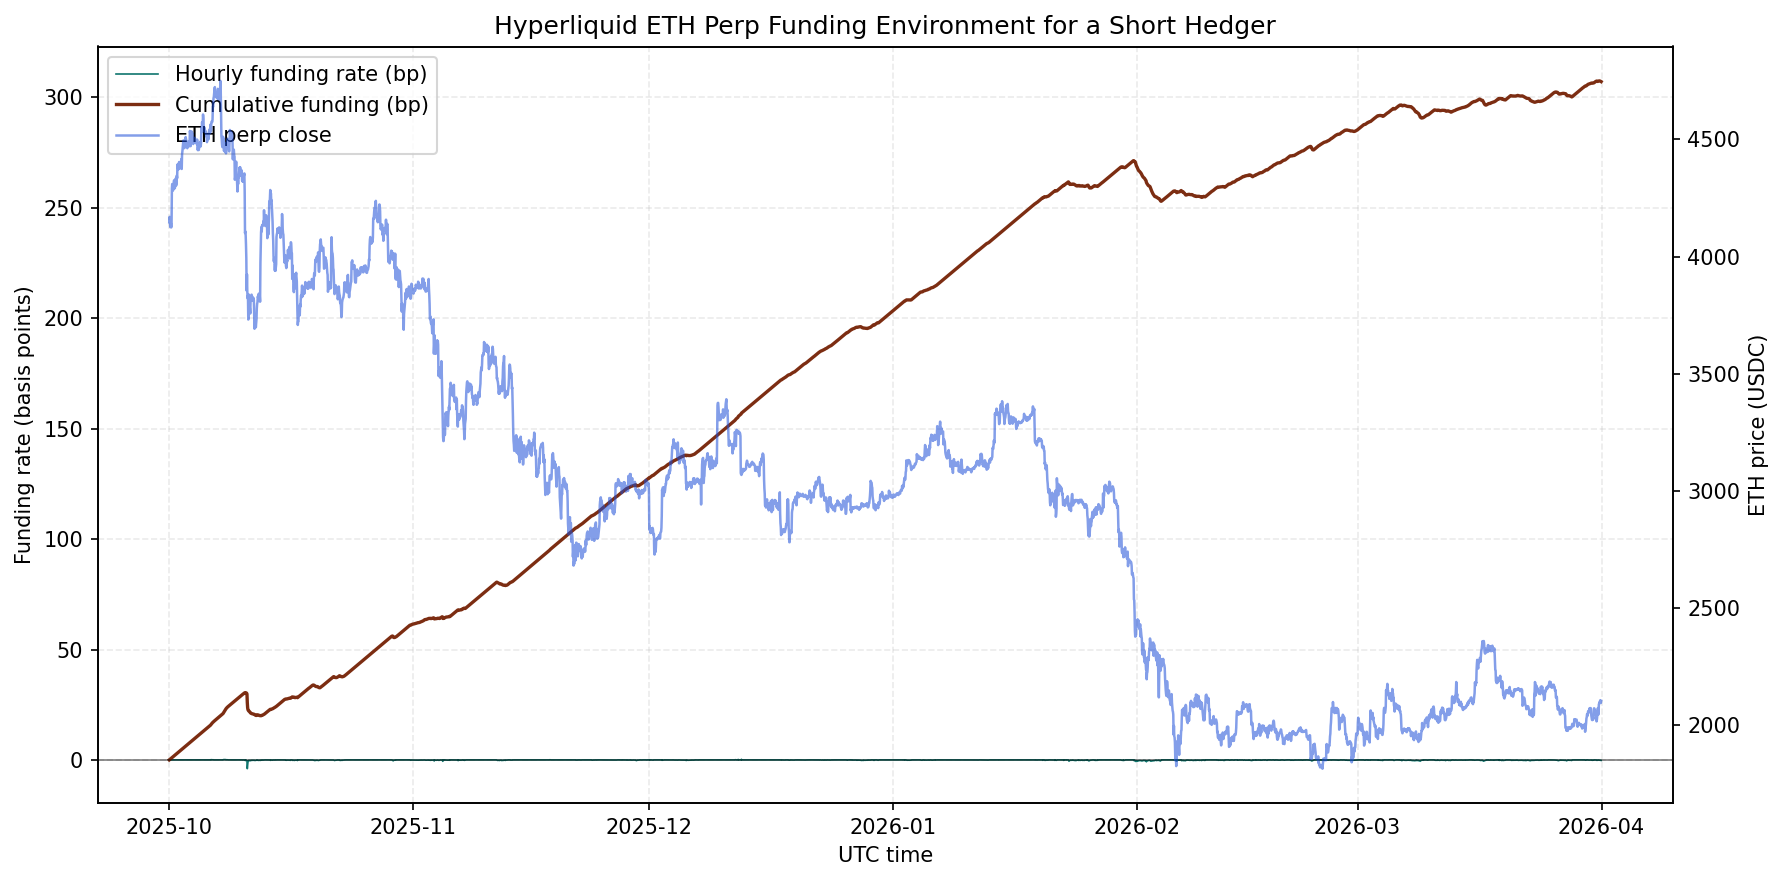
\includegraphics[width=0.9\textwidth]{../data/results/module_5/figures/module5_funding_environment.png}
    \caption{Hourly funding rate and cumulative funding (left axis) vs.\ ETH perp close price
             (right axis) over the full study window.}
    \label{fig:module5-funding}
\end{figure}

\subsection{Delta-Hedging Backtest (Task 5.3)}
\label{sec:module5-backtest}

\paragraph{Strategy.}
At each rebalance event the strategy opens a short ETH perpetual of size
$q_t^{short} = \Delta_{LP}(p_t)$ ETH, offsetting the LP's long WETH exposure.
Between rebalances the size is held static. Three rebalancing frequencies are tested: 1h, 4h,
and 24h, for each of the five LP positions, giving us $5 \times 3 = 15$ strategy variants.

\paragraph{Monte Carlo expected-delta variant.}
As an extension, the fixed hedge size $\Delta_{LP}(p_t)$ is replaced by a forward-looking
target: $q_t^{short} = \mathbb{E}[\Delta_{LP}(p_{t+h}) \mid p_t]$, where the expectation is
estimated by simulating $10{,}000$ GBM paths over the next rebalance horizon $h$.
The rationale is that the current delta will drift before the next rebalance, so targeting
the expected future delta pre-hedges some of that gamma exposure. The same P\&L accounting
and trading-fee structure applies. Results are available in \texttt{hedge\_results.parquet} under
\texttt{strategy = monte\_carlo\_expected\_delta}.

\paragraph{P\&L accounting.}
At each hourly step $t$ the following quantities are computed and accumulated:
\begin{align*}
\text{Hedge P\&L}_t        &= -q_{t-1}^{short}\,(p_t - p_{t-1}),\\
\text{Funding P\&L}_t      &= q_{t-1}^{short}\cdot\mathrm{oracle}_t\cdot f_t,\\
\text{Trading fee}_t       &= 0.00045\cdot|\Delta q_t|\cdot p_t
                              \quad\text{(charged at each rebalance)},\\
\text{Net hedge P\&L}_t    &= \textstyle\sum_{\tau\le t}
                              \bigl(\text{Hedge P\&L}_\tau
                              + \text{Funding P\&L}_\tau
                              - \text{Trading fee}_\tau\bigr).
\end{align*}
At each step the following are also recorded:
\begin{align*}
\text{HODL value}_t      &= x_0\,p_t + y_0,\\
\text{Gross IL}_t        &= \text{HODL value}_t - V_{LP}(p_t),\\
\text{Residual IL}_t     &= \text{Gross IL}_t - \text{Net hedge P\&L}_t,\\
\text{Net position P\&L}_t &= \text{LP fee income}_t - \text{Residual IL}_t,
\end{align*}
where LP fee income is the cumulative swap-fee income from Module 4 (forward-filled from daily
snapshots). All per-step results are stored in \texttt{hedge\_results.parquet}.

\paragraph{Results.}
Figure~\ref{fig:module5-hedge} and Table~\ref{tab:module5-hedge} summarise the terminal net
LP-plus-hedge P\&L for the fixed-frequency schedules.
For concentrated positions (P1, P2), the 4h schedule outperforms 1h because fee savings exceed
the additional gamma drift accumulated between rebalances.
For wider positions (P3, P4), hourly rebalancing limits gamma exposure enough to outperform
the coarser schedules on a net basis.
P5 (the near-full-range position) is largely insensitive to rebalancing frequency.

\begin{figure}[h]
    \centering
    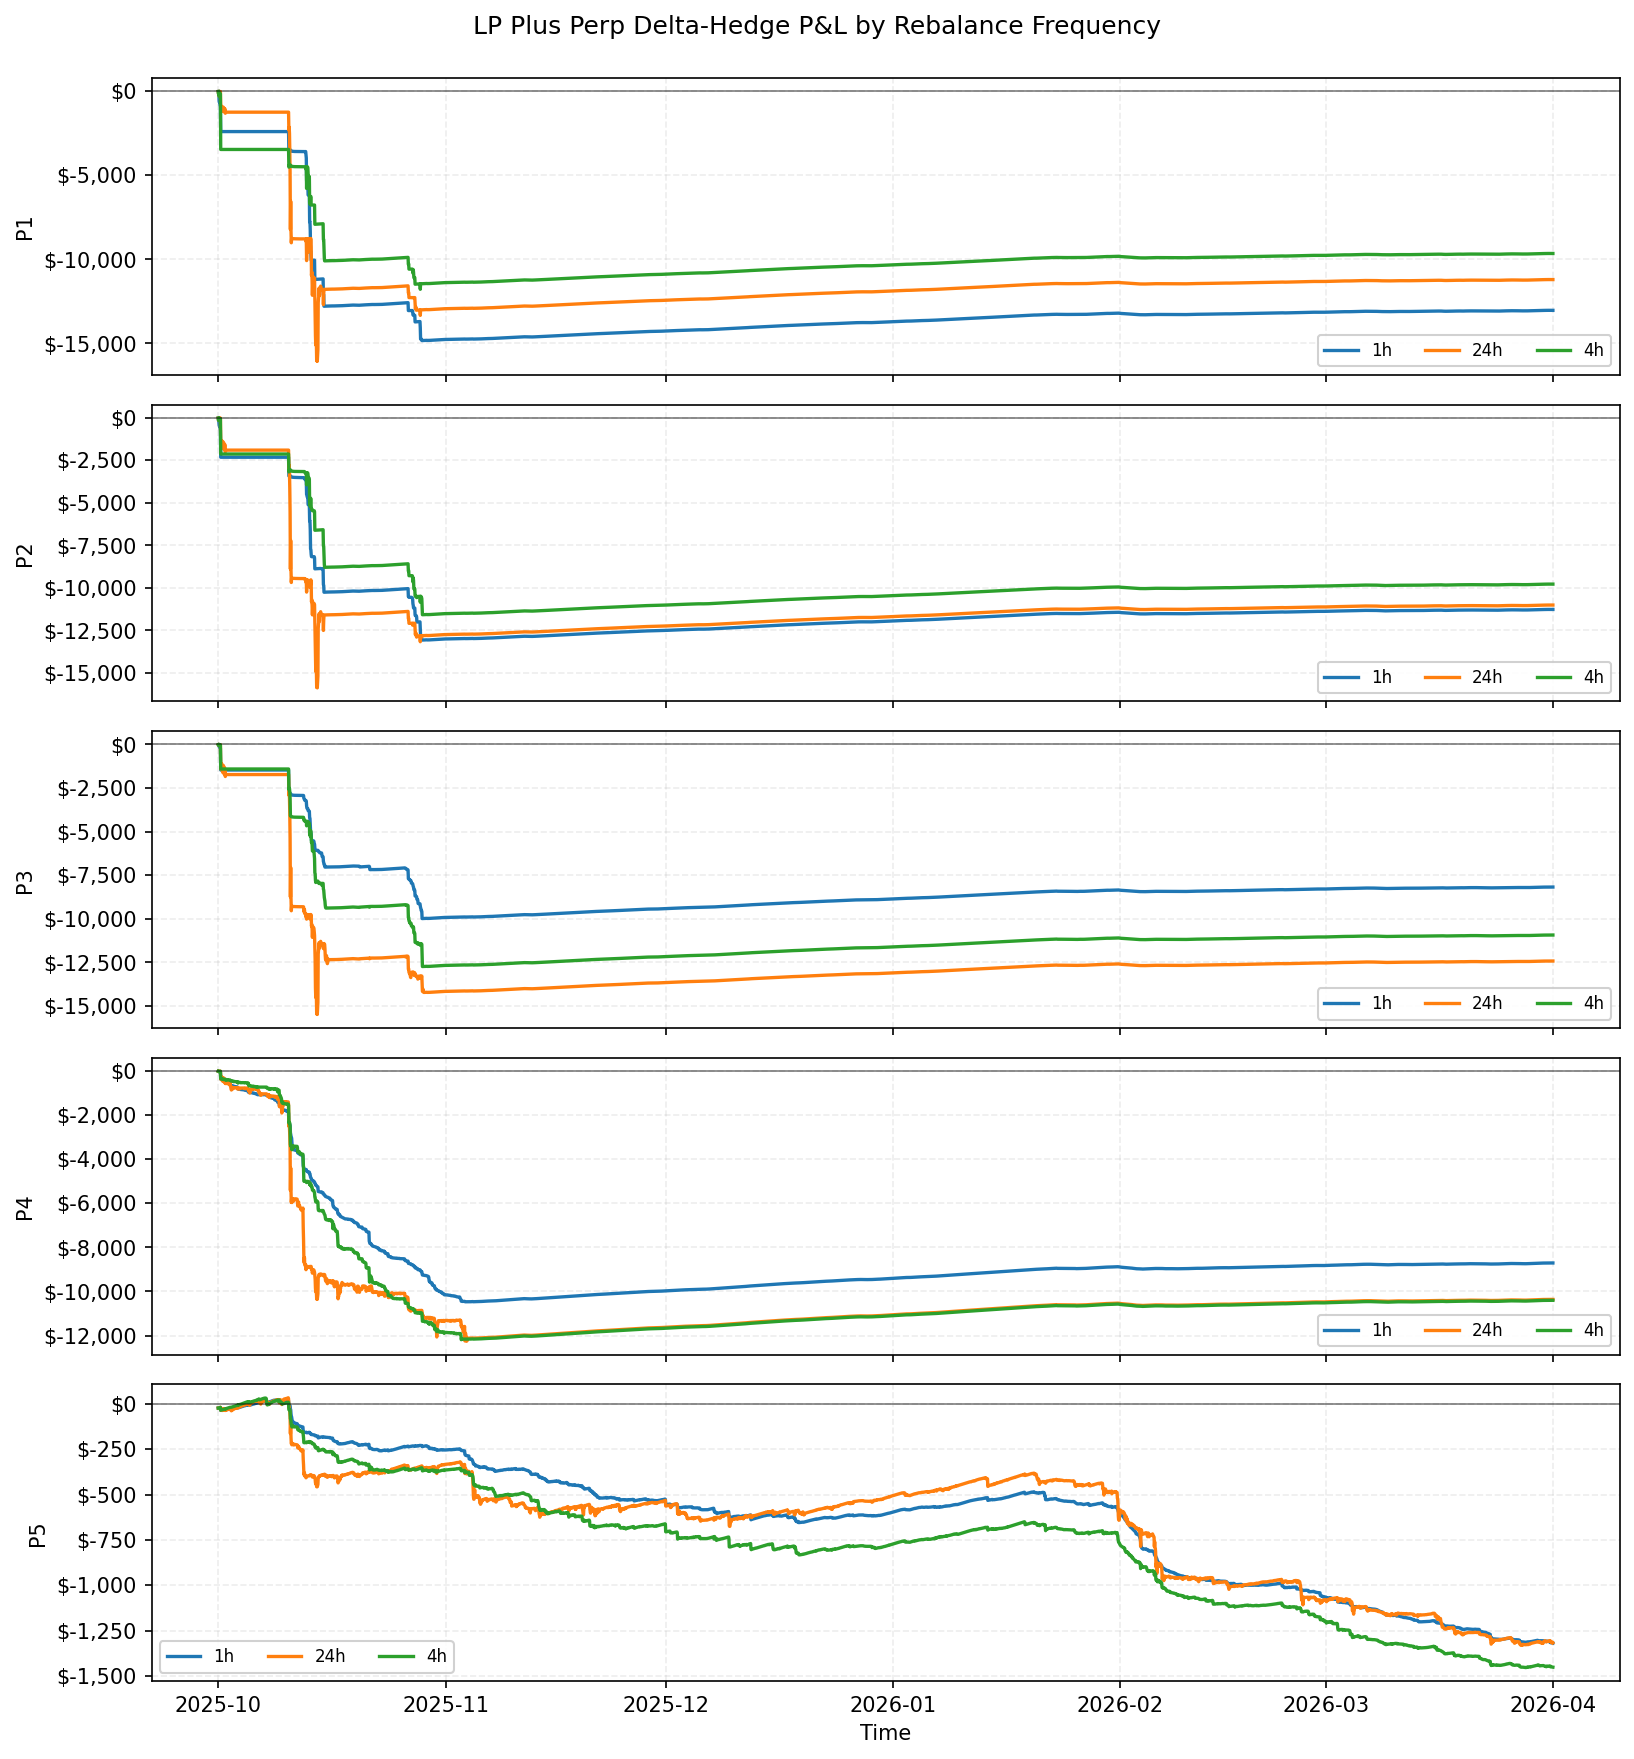
\includegraphics[width=0.95\textwidth]{../data/results/module_5/figures/module5_hedge_results.png}
    \caption{Cumulative net LP-plus-hedge P\&L by position and rebalancing frequency.
             Hedge P\&L, funding income, and trading costs are all included.}
    \label{fig:module5-hedge}
\end{figure}

\begin{table}[h]
\centering
\caption{Terminal net LP-plus-hedge P\&L and cumulative trading fees by position and
         rebalancing frequency (USD).}
\label{tab:module5-hedge}
\small
\begin{tabular}{lrrrrrr}
\hline
 & \multicolumn{2}{c}{1h} & \multicolumn{2}{c}{4h} & \multicolumn{2}{c}{24h} \\
Position & Net P\&L & Fees & Net P\&L & Fees & Net P\&L & Fees \\
\hline
P1 & $-$13\,035 & 967 & $-$9\,652 & 517 & $-$11\,205 & 248 \\
P2 & $-$11\,265 & 994 & $-$9\,777 & 528 & $-$11\,007 & 263 \\
P3 & $-$8\,181  & 754 & $-$10\,931 & 435 & $-$12\,421 & 236 \\
P4 & $-$8\,709  & 854 & $-$10\,402 & 471 & $-$10\,360 & 213 \\
P5 & $-$1\,319  & 220 & $-$1\,452  & 127 & $-$1\,317  &  67 \\
\hline
\end{tabular}
\end{table}

\subsection{Active Exit-Recentering Extension}
\label{sec:module5-active-recenter}

\paragraph{Motivation.}
The fixed-range LPs in Module~4 are passive positions: each range is entered at
the first snapshot and held until the final snapshot. This is a useful benchmark,
but it is not a complete model of active market making. Once the ETH price leaves
a Uniswap V3 range, the position earns no further swap fees and holds one-sided
inventory. A natural active rule is therefore to withdraw and redeploy the same
range width around the current price when the old range is out of range.

\paragraph{Strategy design.}
For each finite-width position P1--P4, the active strategy starts with the same
\$100{,}000 deposit and same width $k$ as Module~4. At each hourly Hyperliquid
timestamp it marks the LP position, accrues swap-fee income from historical
Uniswap swaps whose tick lies inside the current range, and checks whether the
hourly close is outside the range. If it is, the strategy withdraws, pays
rebalancing costs, swaps into the token ratio required by a fresh range, and
redeploys:
\[
[p_a,p_b]=[p_t(1-k),\,p_t(1+k)].
\]
Costs include the 5 bps Uniswap swap fee on the token notional required to
restore the new LP ratio, a \$25 gas estimate per recenter, optional slippage
(set to zero in the baseline), and Hyperliquid taker fees on hedge adjustments.

\paragraph{HODL-tracking hedge.}
The active extension also tests a hedge that tracks the original HODL basket
rather than merely neutralising the LP's ETH delta. Let $E_0$ be the initial WETH
amount of the Module~4 deposit. The signed long ETH hedge target is
\[
q_t = E_0 - \Delta_{LP,t}.
\]
Equivalently, under the code's short-positive convention,
$q_t^{short}=\Delta_{LP,t}-E_0$. The hedge is recomputed after every hourly mark
and after every LP recenter. Performance is measured against the original HODL
benchmark:
\[
\text{Net}_t =
V_{LP,t}+\text{Fees}_t+\text{HedgePnL}_t - V_{HODL,t}.
\]

\begin{figure}[h]
    \centering
    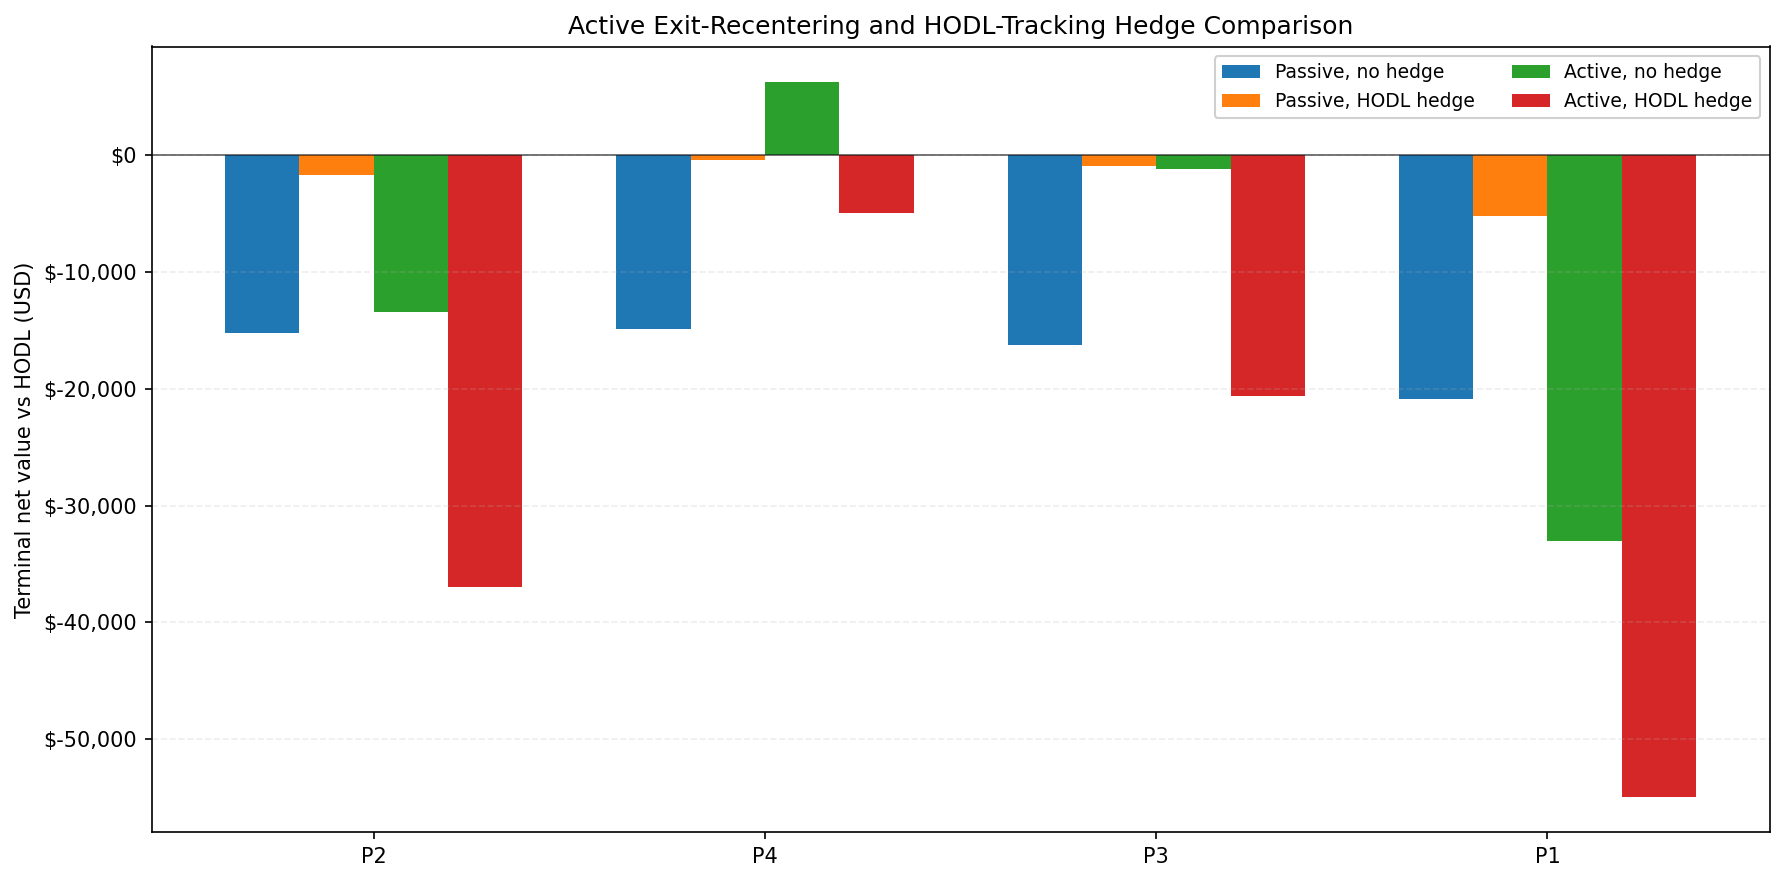
\includegraphics[width=0.95\textwidth]{../data/results/module_5/figures/module5_active_recenter_results.png}
    \caption{Terminal net value versus the original HODL basket for passive fixed-range
             LPs and active exit-recentered LPs, with and without the HODL-tracking hedge.}
    \label{fig:module5-active-recenter}
\end{figure}

\begin{table}[h]
\centering
\caption{Terminal net value versus HODL for passive and active-recentered LP strategies (USD).}
\label{tab:module5-active-recenter}
\small
\begin{tabular}{lrrrr}
\hline
Position & Passive & Passive + hedge & Active & Active + hedge \\
\hline
P1 & $-$20\,886 & $-$5\,209 & $-$33\,002 & $-$54\,936 \\
P2 & $-$15\,203 & $-$1\,645 & $-$13\,447 & $-$36\,968 \\
P3 & $-$16\,257 & $-$858  & $-$1\,166  & $-$20\,584 \\
P4 & $-$14\,894 & $-$384  &  6\,277    & $-$4\,930 \\
\hline
\end{tabular}
\end{table}

The extension shows why re-entering must be interpreted as an active trading
strategy, not as a way to remove IL. Recentering restores fee-earning capacity:
active fee income rises to \$47.4k for P1, \$63.3k for P2, \$72.1k for P3, and
\$38.8k for P4. But the narrow ranges churn heavily. P1 recenters 3,245 times
and pays \$87.9k in LP rebalancing costs; P2 recenters 1,483 times and pays
\$41.8k. Wider ranges rebalance less often: P3 recenters 303 times, while P4
recenters only 17 times and is the only active no-hedge strategy to finish above
HODL in this baseline. The HODL-tracking hedge helps passive fixed ranges during
the downward trend, but it hurts the active recentered strategies here because
the repeated inventory resets and hedge adjustments create path-dependent losses.
Thus re-entering increases fee income, but it also realizes inventory changes and
introduces swap, gas, slippage, and hedge-adjustment costs.

A less reactive threshold rule improves this trade-off. In this variant the LP
recenters only when price has moved at least 50\% of the range half-width from
the current center, a 24-hour cooldown has elapsed, and the trailing 24-hour
in-range fee estimate exceeds the estimated rebalance cost. The hedge is also
made deliberately lazy with a 5 ETH no-trade band. Under this cost-aware rule,
P4 finishes at +\$3.1k versus HODL both with and without the HODL-tracking hedge,
after 57 recenters. The hedge adds almost no value in this case (net hedge P\&L
is -\$37), but it also no longer destroys the strategy. A sensitivity run with a
75\% threshold and 48-hour cooldown gives the strongest unhedged result, P2 at
+\$24.0k versus HODL and P4 at +\$7.2k, but the hedged versions remain weaker.

\subsection{Limitations and Critical Discussion (Task 5.4)}
\label{sec:module5-limitations}

\paragraph{Residual gamma risk.}
A short perpetual cancels today's delta but does not remove curvature. Between rebalances the
hedge drifts from the true delta by an amount driven by $\Gamma_{LP}$; the resulting convexity
loss is approximated by $\frac{1}{2}\Gamma_{LP}(p_t)(\Delta p_t)^2$ accumulated over all hours.
This proxy totals $-\$2{,}496$ (P1), $-\$7{,}723$ (P2), $-\$9{,}521$ (P3), $-\$9{,}845$ (P4),
and $-\$2{,}444$ (P5). Narrow positions carry the highest gamma exposure per dollar because they
require larger $L$; infrequent rebalancing compounds this by allowing larger inter-period price
moves.

\paragraph{Funding-rate risk.}
Over the study window the mean hourly funding rate is $7.3\times10^{-6}$, providing the short
hedger a small persistent credit. During the 219 large-move hours (absolute log return above the
95th-percentile threshold of $1.52\%$), the mean rate drops to $1.7\times10^{-6}$: funding
income is smallest precisely when gamma losses are largest. This adverse correlation means
funding receipts do not reliably cushion the worst impermanent-loss events.

\paragraph{Minimum viable position size.}
Cumulative trading fees under the 1h schedule range from \$220 (P5) to \$994 (P2) over six
months. An LP must earn enough in swap fees to cover these costs plus any residual IL. Positions
whose expected fee income falls short of this threshold cannot justify continuous 1h rebalancing;
switching to 4h or a no-trade-band schedule reduces the fee burden by 40--50\%, lowering the
break-even notional accordingly.

\paragraph{Options as an alternative hedge.}
A perpetual hedges delta but not gamma. A short-dated ETH put spread or straddle with strikes
at the position's range boundaries would directly offset the concavity left unhedged by the
perpetual, eliminating residual gamma risk entirely. The key assumptions required are
sufficient options liquidity at the relevant strikes and tenors, and that implied volatility at
the time of purchase is below the realised volatility over the hedge horizon, otherwise the
option premium exceeds the gamma loss it prevents. With annualised realised volatility at
$69\%$ over this study window, options merit serious consideration for the most concentrated
positions, P1 and P2, where the gamma proxy exceeds \$2{,}500 and \$7{,}700 respectively.
